\chapter{Deep Learning Overview}\label{chap:dlo}

\localtableofcontents

\section{Introduction}

Deep learning is a subfield of machine learning that focuses on the study of
\acp{DNN}. \acp{DNN} are a family of machine learning algorithms that have their
roots in \acp{ANN} which aim to learn a data representation from unstructured
data such as raw images \cite{DBLP:conf/nips/KrizhevskySH12}, text
\cite{DBLP:conf/emnlp/BudzianowskiV19} or audio
\cite{DBLP:journals/corr/HannunCCCDEPSSCN14}, in an end-to-end fashion.
\acp{ANN} were initially conceptualised based on the understanding of biological
neural networks present in the brain
\cite{mcculloch1943logical,hebb2005organization}.
\citeauthor{rosenblatt1958perceptron} proposed in
\cite{rosenblatt1958perceptron} a theoretical model of a neuron, denoted the
\emph{perceptron}, which was capable of learning a linear decision boundary. The
perceptron model was later extended to multiple layers of neurons, giving rise
to the \ac{MLP} \cite{rosenblatt1961principles,rumelhart1986learning}. A
\acl{MLP} is a type of artificial neural network that extends the concept of a
single-layer perceptron by including one or more hidden layers of neurons
connected upstream to an input layer and downstream to an output layer. Each
layer is fully connected to the next, allowing the model to learn and represent
more complex, non-linear relationships in the input data. Although able to learn
more complex boundaries than the perceptron, the \ac{MLP} is still limited by
its depth. The next advance came from the stacking of multiple layers, leading
to \aclp{DNN}.\\

In the context of \acp{DNN}, the term \emph{deep} denotes the stacking of many
layers within a neural network. The concept of \acp{DNN} is based on the idea
that the depth and the numerous layers can help in learning features at various
levels of abstraction, enabling the network to learn complex hierarchical
patterns. For instance, in the context of image recognition, lower layers may
learn local features like edges and textures, while deeper layers might learn to
identify more abstract concepts like shapes or objects.\\

The rise of \acp{DNN} was made possible by several factors. On the one hand the
increase in computational power, and in particular the use of \acp{GPU}, which
made the training of deep networks feasible. Indeed, AlexNet, the first \ac{CNN}
to win the ImageNet Large Scale Visual Recognition Challenge
\cite{DBLP:conf/nips/KrizhevskySH12}, was trained on two \acp{GPU} in parallel
to accelerate computations. Nowadays, the use of \acp{GPU} or dedicated hardware
such as \acp{TPU} is ubiquitous and supported by all the major deep learning
frameworks
\cite{DBLP:journals/corr/AbadiABBCCCDDDG16,DBLP:conf/nips/PaszkeGMLBCKLGA19}.On
the other hand, the availability of large-scale datasets such as ImageNet
\cite{deng2009imagenet} allowed to train or pre-train deep networks with
millions of parameters without overfitting.\\

This chapter aims to give an overview of the different neural network
architectures, building blocks, training techniques and datasets that are widely
used in Deep Learning for computer vision as well as our experiments.
\Cref{sec:dlo:early_architectures} introduced the early neural network
architectures, namely the perceptron and the \ac{MLP}. \Cref{sec:dlo:training}
focuses on the functional definition of a neural network and its training.
\Cref{sec:dlo:cnn} presents the building blocks and architectures of various
\acp{CNN} for computer vision, and finally, \Cref{sec:dlo:datasets} gives an
overview of the datasets used in our experiments.
% TODO: rafiner cette partie

% In the context of \acp{DNN}, the term \emph{deep} denotes the stacking of many
% layers within a neural network. A \ac{DNN} consists of layers, each layer is an
% operation that takes information from the previous layers, processes it and then
% passes it on through an activation function
% \cite{glorot2011deep,DBLP:journals/pieee/LeCunBBH98,klambauer2017self} that
% introduce non linearity. Finally, this output is sent to the next layer. Among
% the most fundamental types of these layers are \emph{Convolutional} and
% \emph{Dense} (or fully connected) layers. \\

\section{Early architectures}\label{sec:dlo:early_architectures}

In this section, we present the perceptron \cite{rosenblatt1958perceptron} and
then the \acl{MLP} \cite{rosenblatt1961principles,rumelhart1986learning}. Both
are the two founding neural network architectures that led to the development of
\aclp{DNN}.

\subsection{Perceptron}\label{sec:dlo:perceptron}

The \emph{perceptron} is a model of artificial neuron, capable of learning a
linear decision boundary. It was proposed by
\citeauthor{rosenblatt1958perceptron} in 1958 \cite{rosenblatt1958perceptron}
and conceptualised based on the understanding of biological neural networks
present in the brain \cite{mcculloch1943logical,hebb2005organization}. The
perceptron is composed of inputs that are weighted and summed before being
passed through an nonlinear function refered to as an activation function. The
conceptrual representation of the perceptrion is displayed in
\cref{fig:dlo:perceptron} and its mathematical formulation is defined in
\cref{eqn:dlo:perceptron}: \\
% and can be express in vector form as written in \cref{eqn:dlo:perceptron_vector}.\\

\begin{equation}
  \label{eqn:dlo:perceptron}
\hat{y} = g(\sum_{i=1}^{n} w_i \cdot x_i + b)
\end{equation} \\


% \begin{equation}
%   \label{eqn:dlo:perceptron_vector}
%   \hat{y} = g(\mathbf{w}^T \mathbf{x} + b)
% \end{equation}\\

\noindent where $x_i$ is the $i$th input, $w_i$ is the weight associated with
the $i$th input,$n$ is the number of inputs, $b$ is the bias, $g$ is the
activation function, and $\hat{y}$ is the perceptron's output. The activation
function is typically a nonlinear function, such as the sigmoid function or the
hyperbolic tangent function. Due to its shallow architecture, the perceptron
cannot learn complex decision boundaries. Nevertheless, it is possible to stack
several perceptrons to learn nonlinear decision boundaries, leading to a
\acl{MLP}.\\

\begin{figure}[htbp]
  \centering
  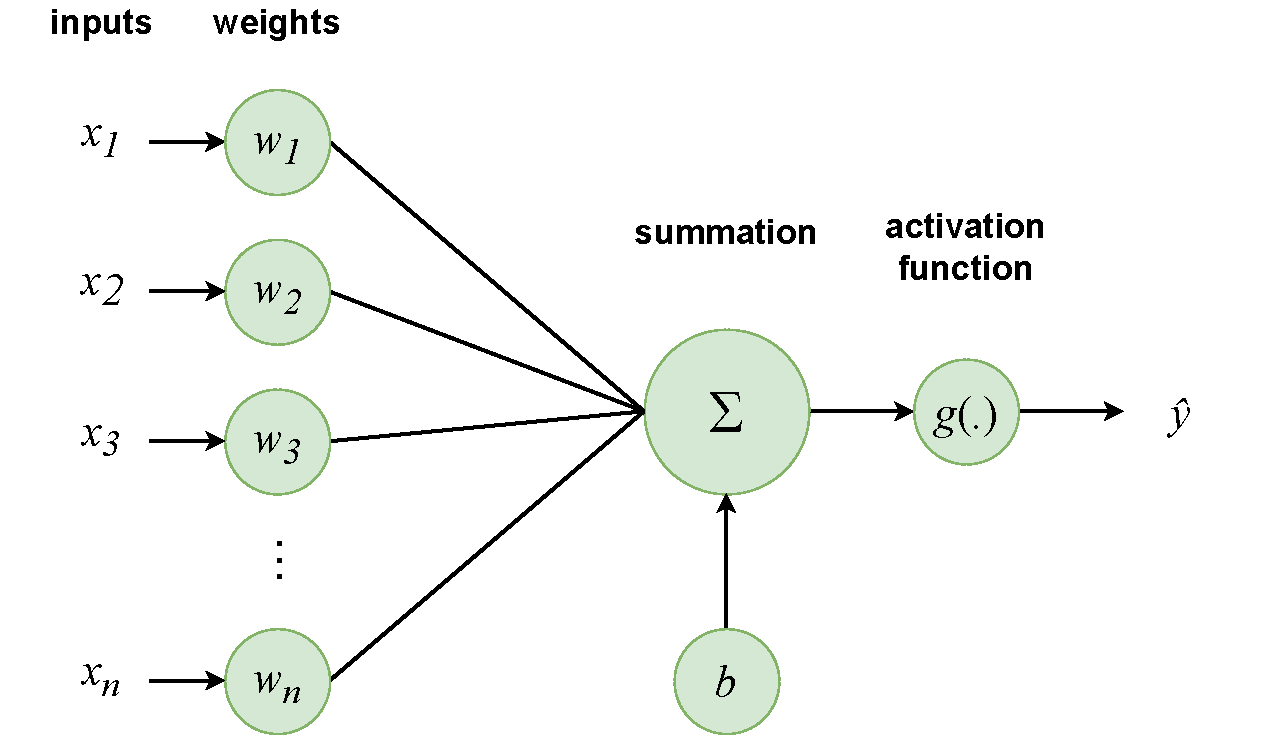
\includegraphics[width=0.7\textwidth]{chapter_dlo/assets/perceptron_scheme.pdf}
  \caption{Conceptual scheme of the \emph{perceptron}. Each input $x_i$ is multiplied
  by its associated weight $w_i$ and summed to the other weighted inputs. The
  bias $b$ is added to the sum and the result is passed through an activation
  function $g$ to produce the output $\hat{y}$.}
  \label{fig:dlo:perceptron}
\end{figure}

\subsection{Multilayer Perceptron}\label{sec:dlo:mlp}


The \acf{MLP} is an extension of the perceptron model, comprising multiple
layers of perceptrons, also referred to as neurons \cite{rumelhart1986learning}.
A \ac{MLP} with one hidden layer is represented in \cref{fig:dlo:mlp}. In the
latter, the circles represent the neurons, and the connections between
representing weights are materialised by lines. The \ac{MLP} is the simplest
type of feedforward \ac{ANN}. Feedforward refers to the fact that the
connections between neurons in the \ac{MLP} form a \acf{DAG}, where the outputs
of the neurons from one layer are passed to the next, with no backward
connections.\\

Each layer of the \ac{MLP} being fully connected to the next one, it enables the
\ac{MLP} to handle problems that the perceptron cannot solve, such as problems
requiring nonlinear decision boundaries. Furthermore,
\citeauthor{cybenko1989approximation} proved in \cite{cybenko1989approximation}
that an \ac{MLP} can approximate continuous functions on compact subsets of
$\mathbb{R}^n$. This result is known as the \emph{Universal Approximation
Theorem}, also known as \emph{Cybenko Theorem}. Before the emergence of Deep
Learning, \acp{MLP} have been applied to various domains, including voice
recognition, image recognition, and machine translation
\cite{wasserman1988neural}.


\begin{figure}[htbp]
  \centering
  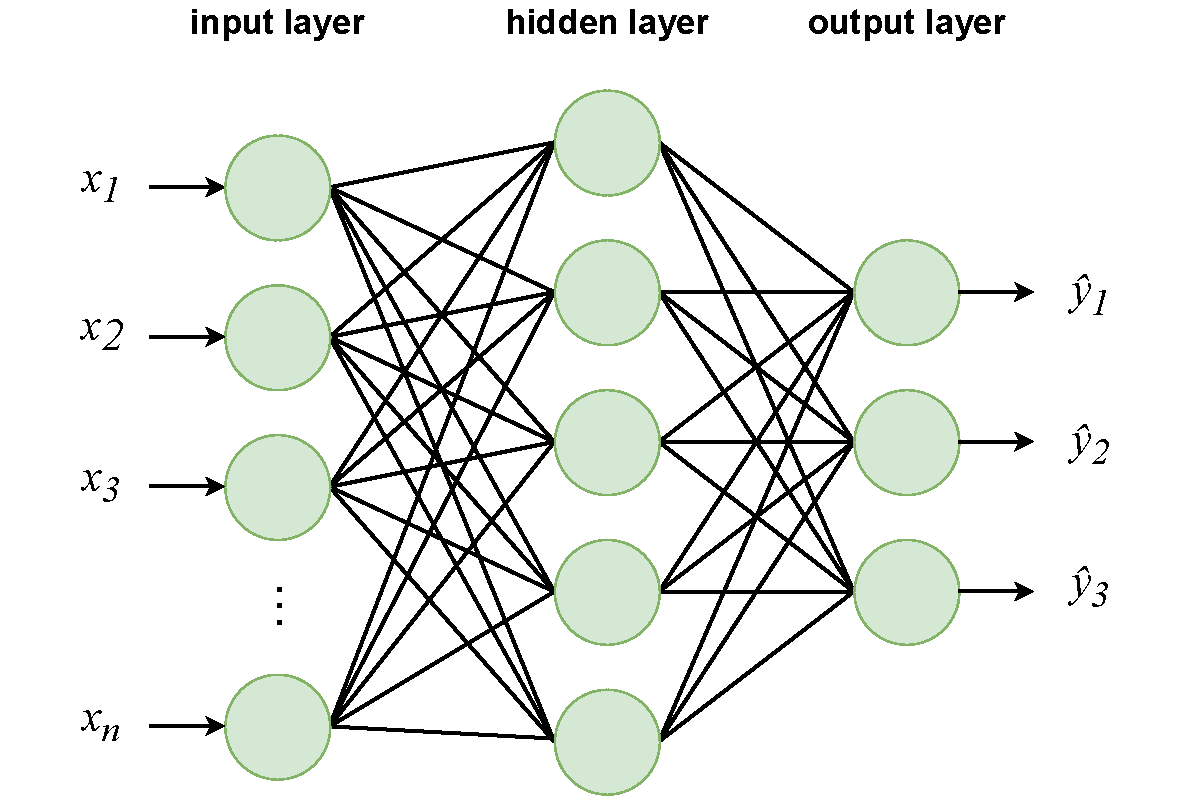
\includegraphics[width=0.7\textwidth]{chapter_dlo/assets/mlp_scheme.pdf}
  \caption{\ac{MLP} scheme}
  \label{fig:dlo:mlp}
\end{figure}

\section{Training}\label{sec:dlo:training}
\subsection{Functional definition}
\subsection{Loss function and regularisation}
\subsection{Optimisation through backpropagation}

\section{Convolutional Neural Networks for Computer Vision}\label{sec:dlo:cnn}
\subsection{Building Blocks}
\subsection{Architectures}

\section{Datasets}\label{sec:dlo:datasets}

In this thesis manuscript, we focuses on image classification tasks and
supervised learning. Supervised learning is a machine learning paradigm in which
the model is trained using labelled data. In the context of image
classification, the input data is an image, and the label is the class of the
image. We denote an input image $X$ and its corresponding label $y$. Each image
$X$ belongs to the set of all images of the dataset $\mathcal{X}$, and each
label $y$ belongs to the set of all labels of the dataset $\mathcal{Y}$. The
dataset, denoted $\mathcal{D}$, is a set of pairs $(X, y)$, where $X \in
  \mathcal{X}$ and $y \in \mathcal{Y}$, so that $D \subset \mathcal{X} \times
  \mathcal{Y}$. \\

In our experiments, we evaluated our methods on three different datasets
tailored for image classification: CIFAR-10 \cite{CIFARdataset}, CIFAR-100
\cite{CIFARdataset} and TinyImageNet \cite{TinyImageNet}. The following
paragraphs give details about these datasets and \cref{tab:dlo:datasets} sums
up their main characteristics.\\

\begin{table}[ht!]
  \centering
  \begin{tabular}{lcccc}
    \toprule
    \textbf{Dataset}    & \textbf{Number of images} & \textbf{Number of classes} &
    \textbf{Image size} & \textbf{Size of test set}                                               \\
    \hline
    CIFAR-10            & 60,000                    & 10                         & 32x32 & 10,000 \\
    CIFAR-100           & 60,000                    & 100                        & 32x32 & 10,000 \\
    TinyImageNet        & 100,000                   & 200                        & 64x64 & 10,000 \\
    \bottomrule
  \end{tabular}
  \caption{The number of images, of classes, image size and size of the test
    set for the three datasets used: CIFAR-10, CIFAR-100 and TinyImageNet.}
  \label{tab:dlo:datasets}
\end{table}

\subsection{CIFAR-10}

The CIFAR-10 dataset \cite{CIFARdataset} is a widely
used dataset in machine learning and computer vision. This is a labeled subset
of the \emph{80 Millions Tiny Images} dataset \cite{4531741}. CIFAR-10 is a
simple yet challenging dataset that allows for quicker iteration or
hyperparameter tuning than larger datasets such as ImageNet
\cite{DBLP:journals/ijcv/RussakovskyDSKS15}, but it is significanly more complex
than the MNIST dataset \cite{6296535}, which contains grayscale handwritten
digits images. the CIFAR-10 dataset contains 60,000 colour images of size 32x32
pixels, split into 10 classes, namely: plane, car, bird, cat, deer, dog, horse,
ship, truck. Each class contains 6,000 images. The dataset is divided into two
sets: a training set, composed of 50,000 images and a test set containing 10,000
of them.\\

\begin{figure}[ht!]
  \centering
  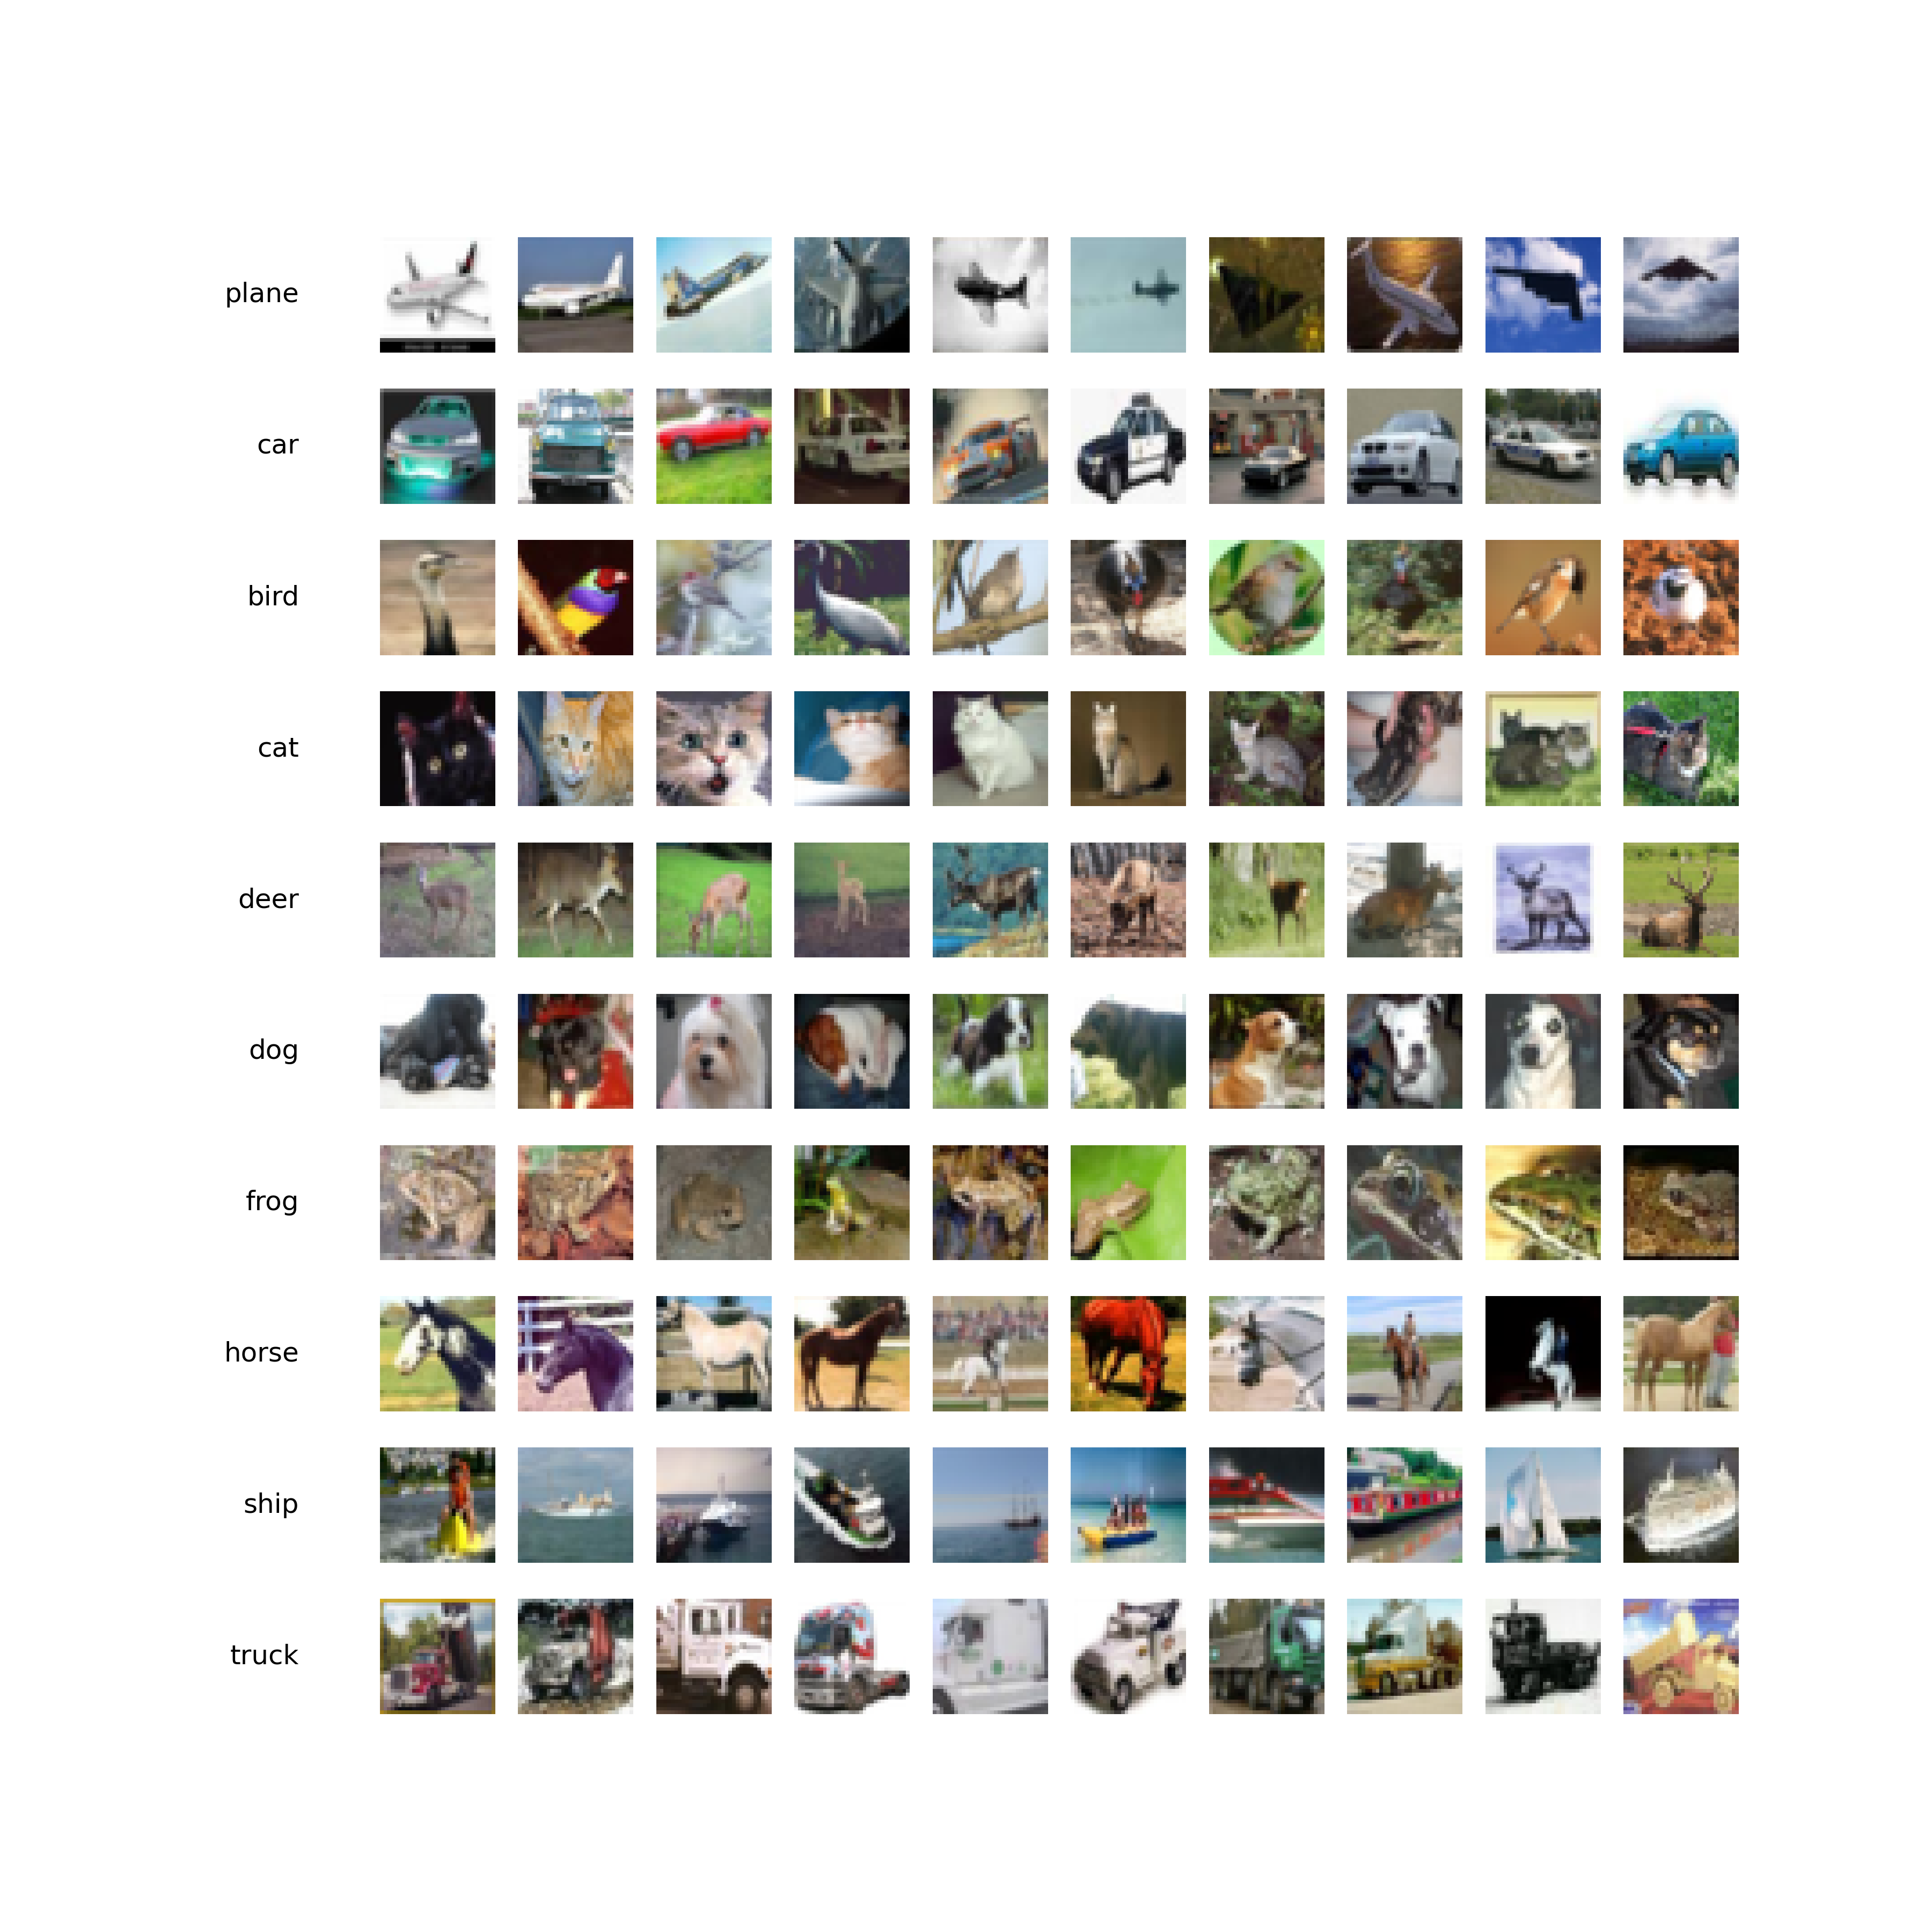
\includegraphics[width=0.7\textwidth]{chapter_dlo/assets/cifar-10_example.png}
  \caption{ A sample grid of images from the CIFAR-10 dataset. Each row
    contains images from one of the 10 classes: plane, car, bird, cat,
    deer, dog, frog, horse, ship, and truck}
  \label{fig:intro:cifar10_examples}
\end{figure}


\subsection{CIFAR-100}

CIFAR-100 \cite{CIFARdataset} is a more challenging
version of CIFAR-10. Like the latter, it is a labeled subset of the \emph{80
  Millions Tiny Images} and  is composed of 60,000 colour images of size 32x32
pixels. However, instead of 10 classes, CIFAR-100 contains 100 classes of 600
images each. As a result, each class has far fewer images than in CIFAR-10.
CIFAR-100 is also divided into two sets: a training set and a test, composed of
50,000 and 10,000 images respectively.\\

\begin{figure}[ht!]
  \centering
  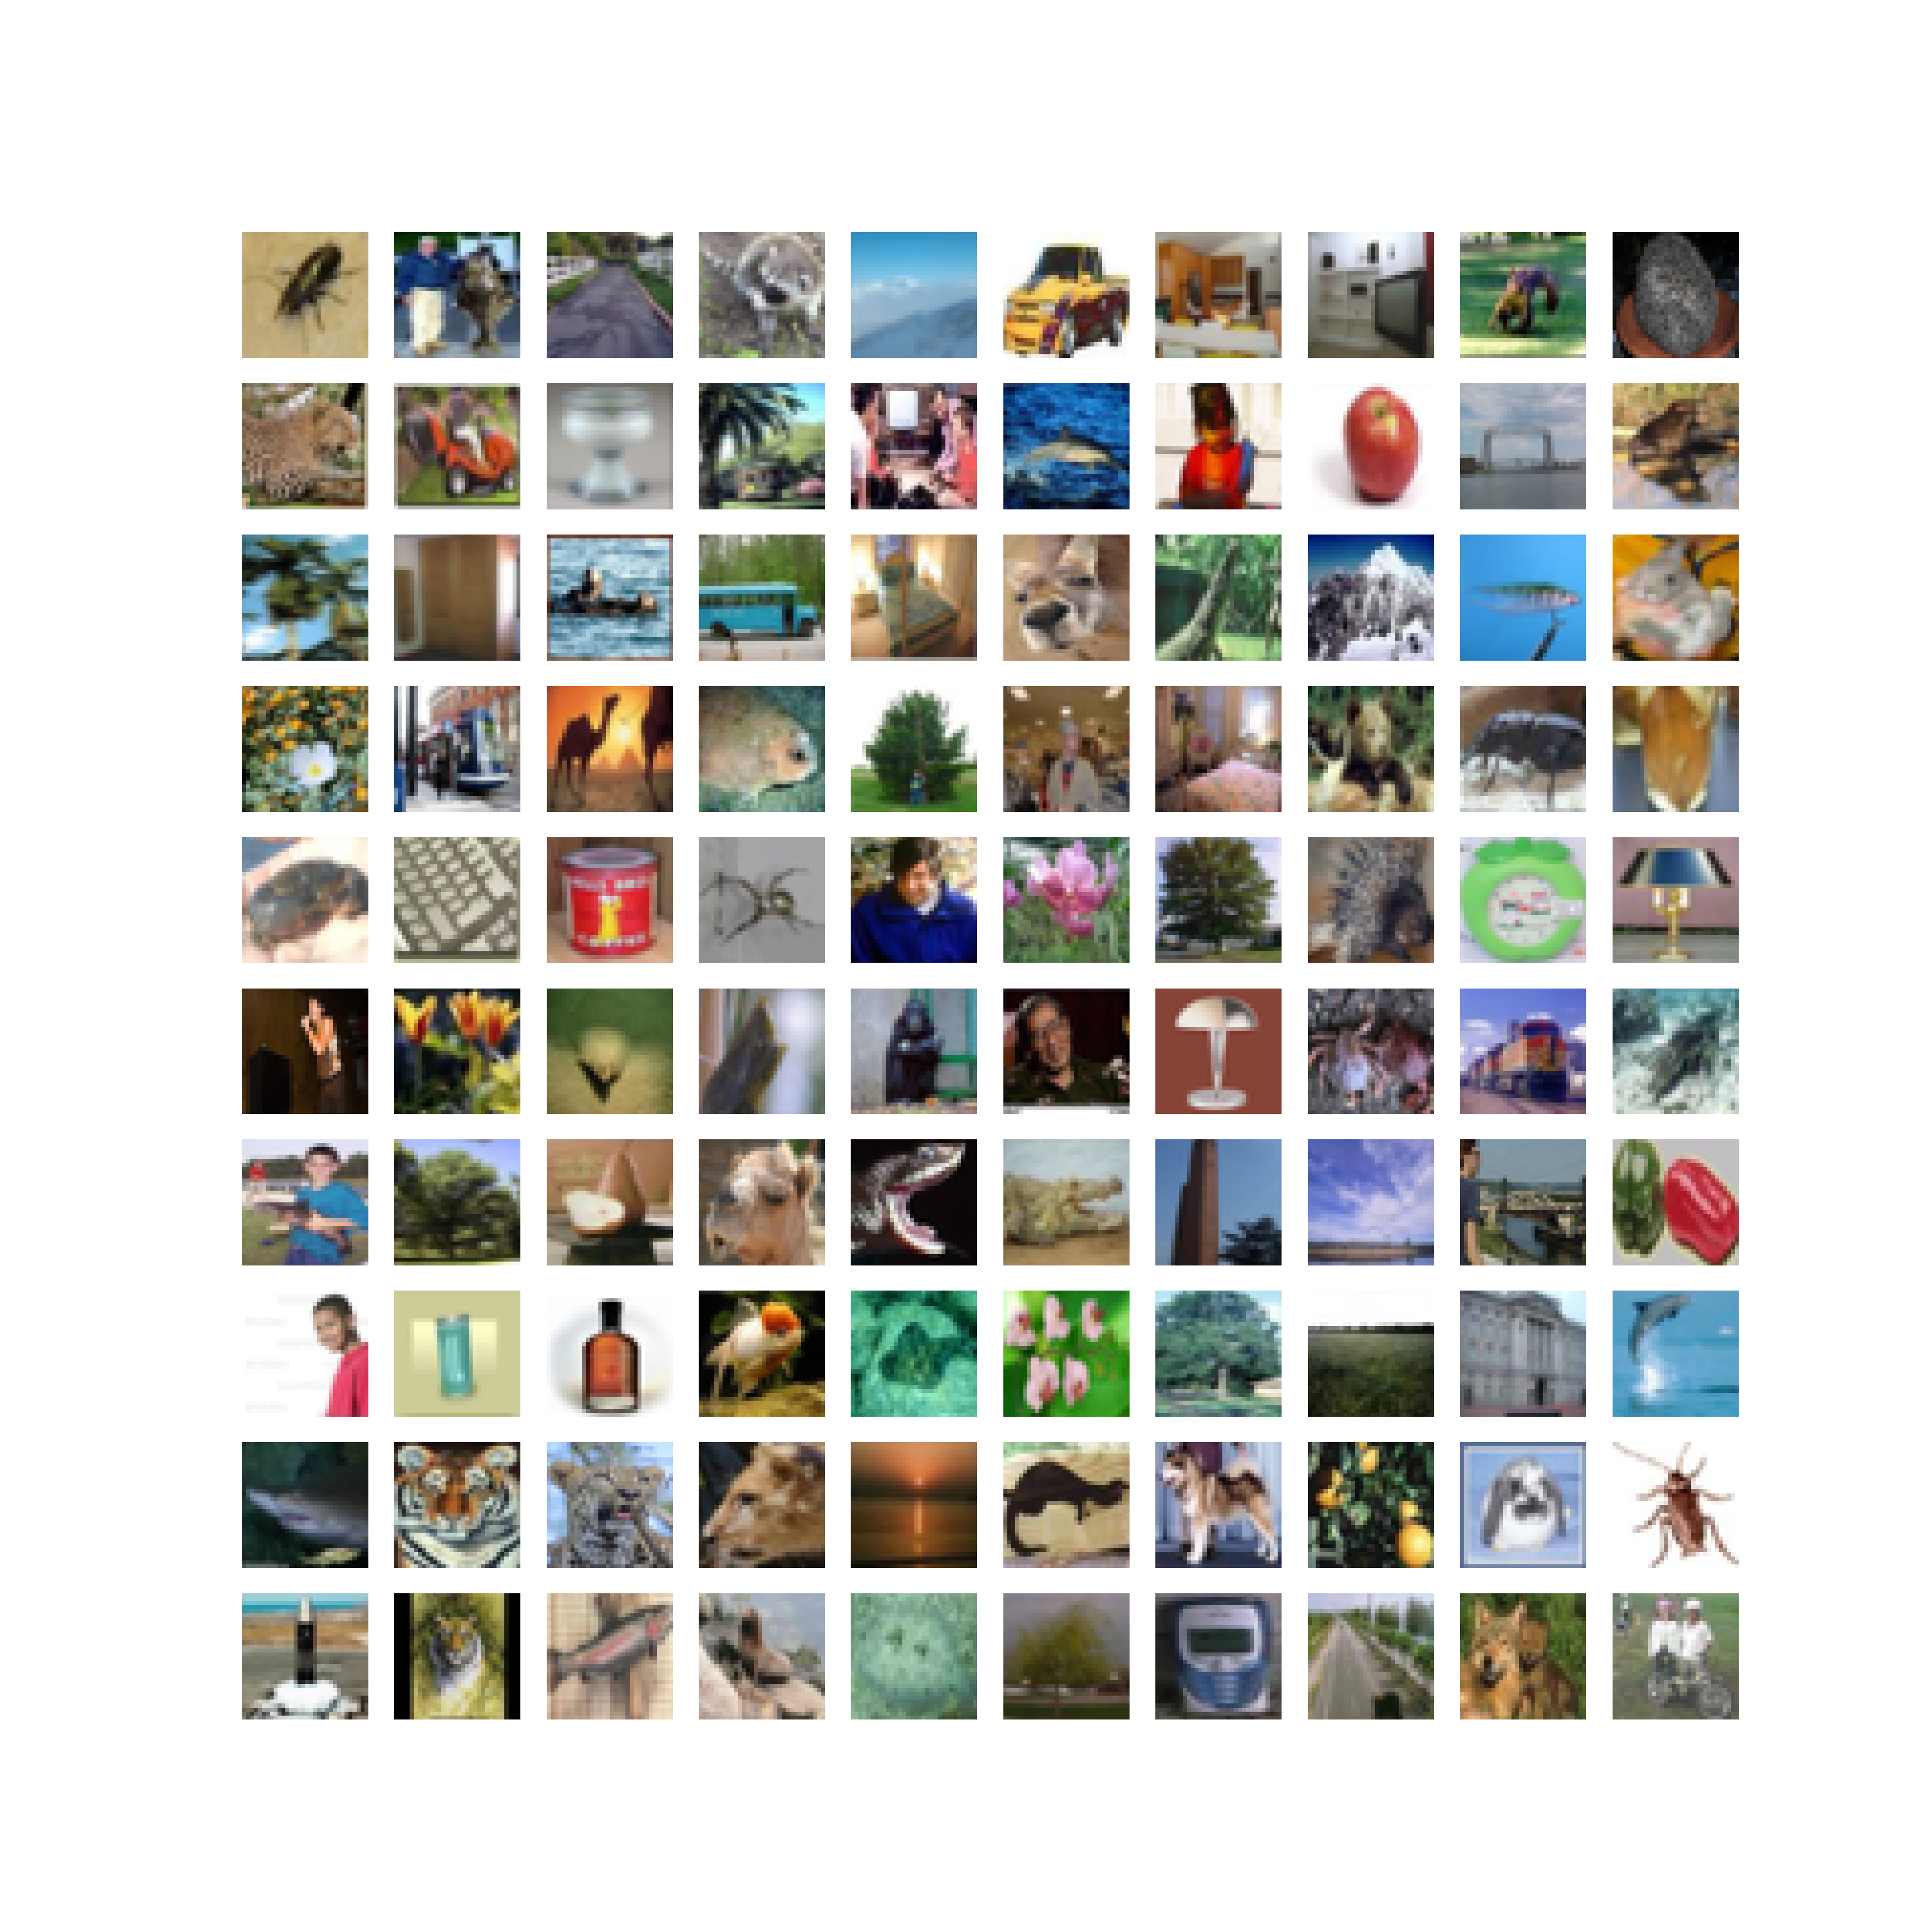
\includegraphics[width=0.7\textwidth]{chapter_dlo/assets/cifar-100_example.png}
  \caption{A sample grid of images from the CIFAR-100 dataset. The images
    represent a subset of the 100 available classes, each image represents
    a unique class.}
  \label{fig:intro:cifar100_examples}
\end{figure}


\subsection{TinyImageNet}

TinyImageNet dataset is another popular dataset
in machine learning and computer vision, conceived as a subset of the larger
ImageNet dataset \cite{DBLP:journals/ijcv/RussakovskyDSKS15}. It comprises
100,000 colour images of size 64x64 pixels, split into 200 classes, whereas
ImageNet contains 1.2 million images of size 256x256 pixels, split into 1,000
classes. The dataset is divided in 3 sets: the train set, containing 500
images per class, the validation and test sets, both containing 50. The scaled
down image size and count make TinyImageNet more computationally accessible than
ImageNet while still being a challenging task and maintening the diversity of
the images and classes.\\


\begin{figure}[ht!]
  \centering
  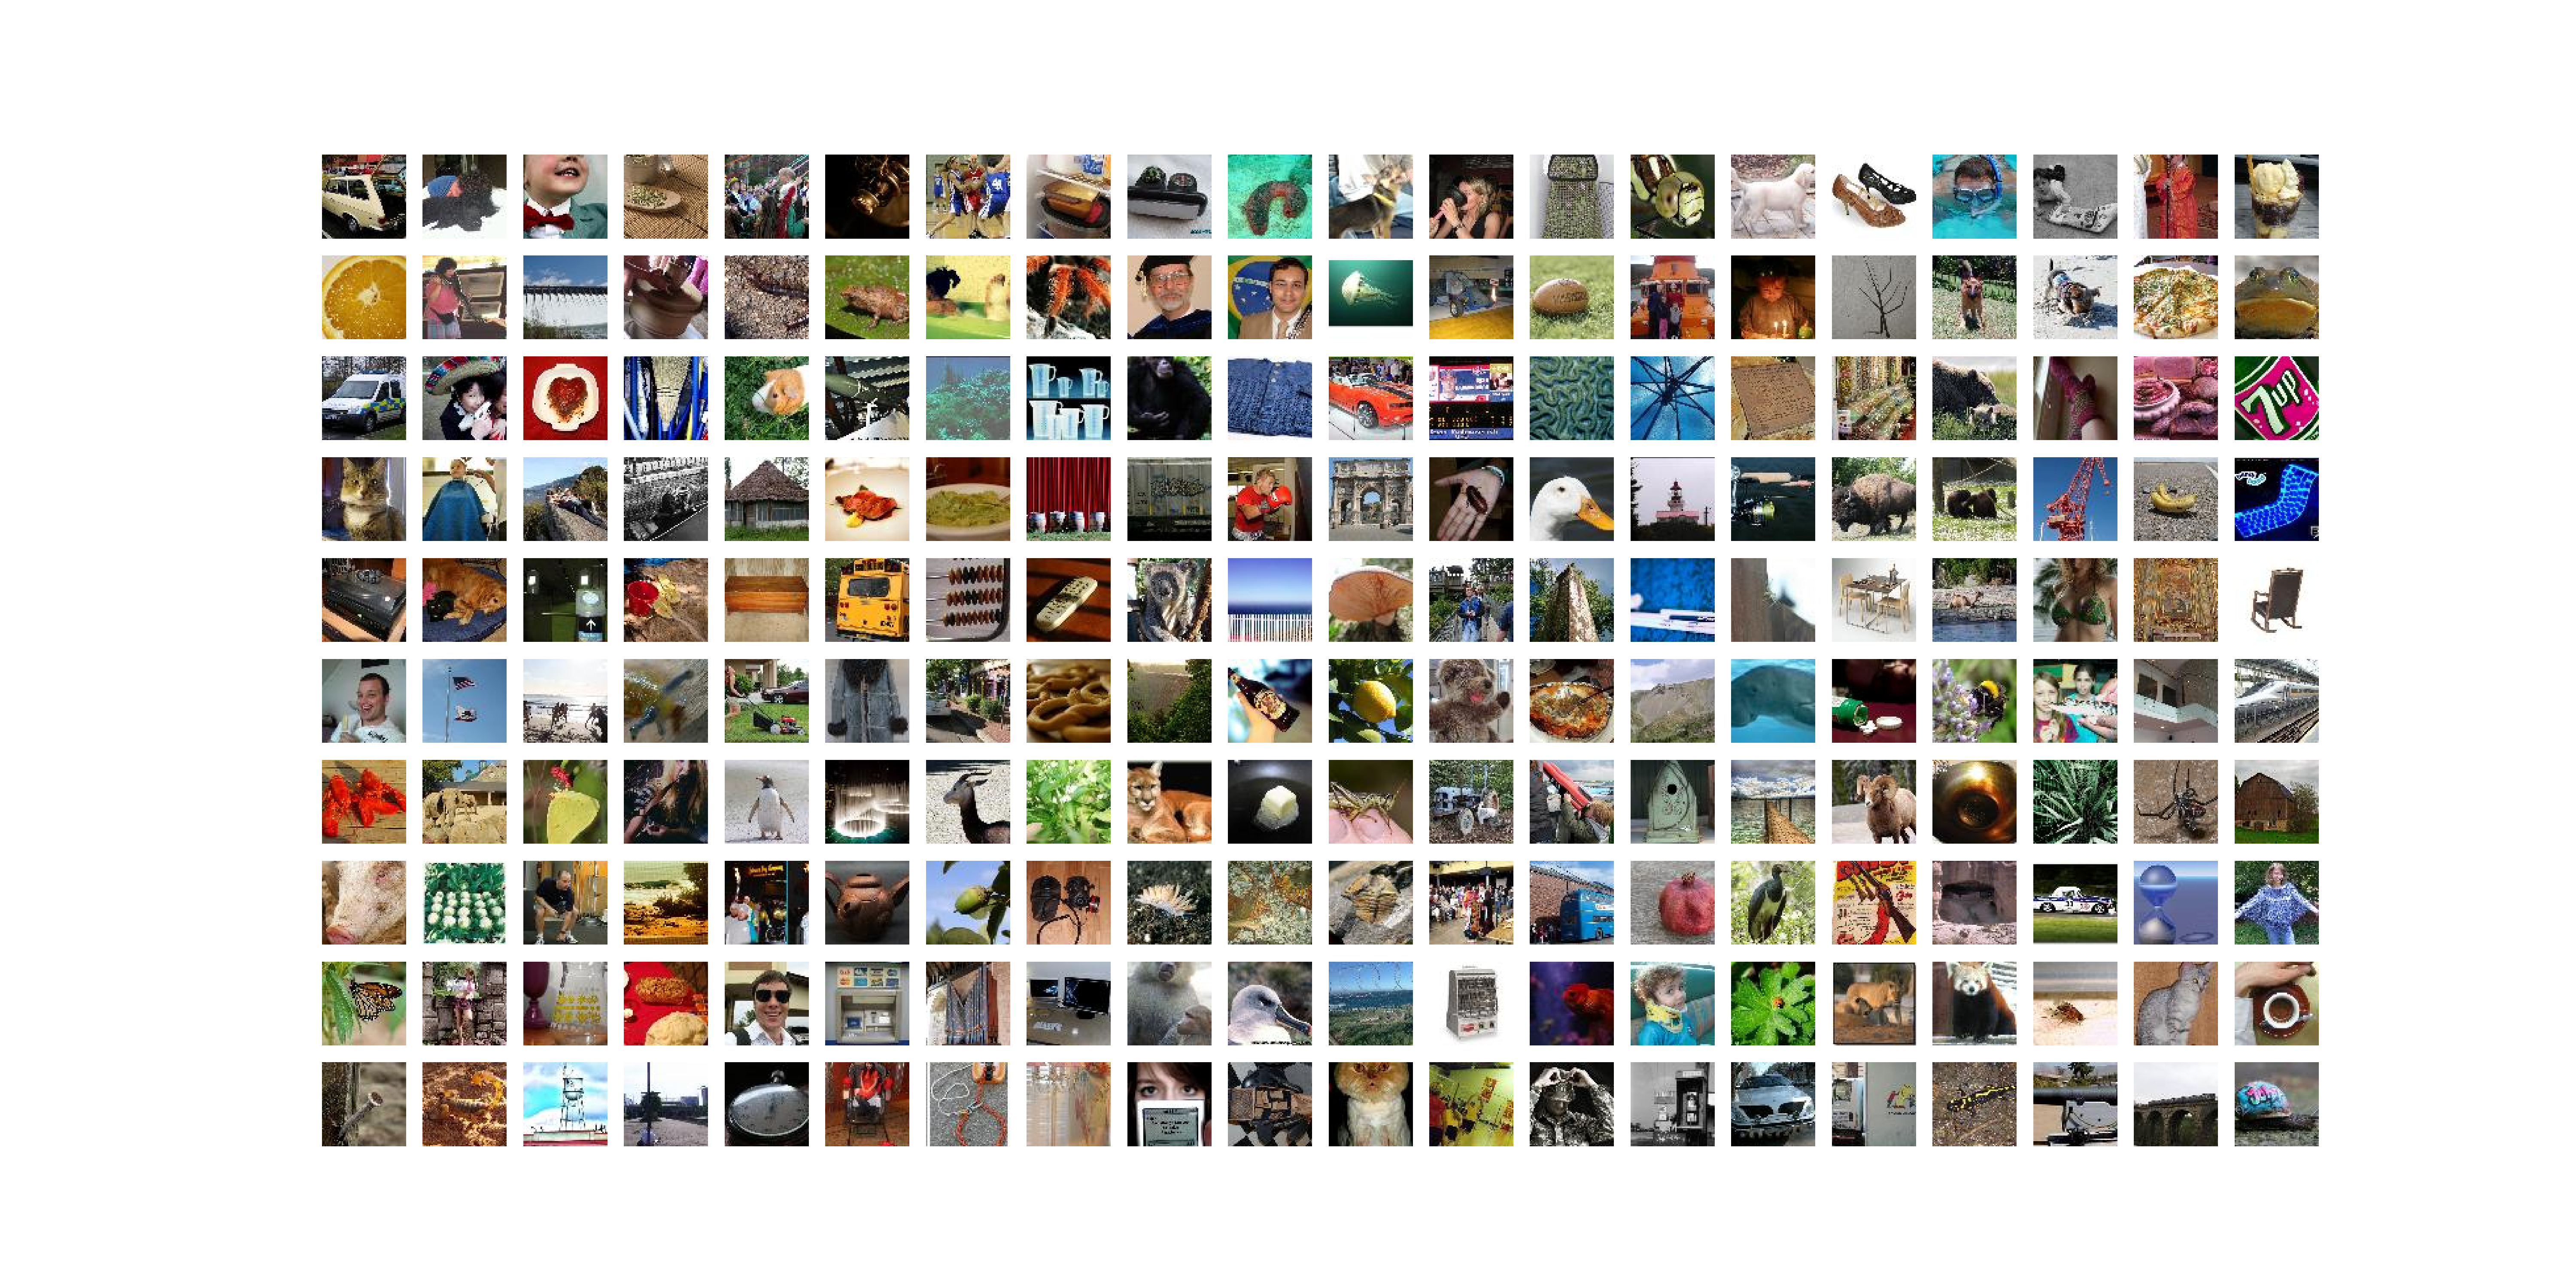
\includegraphics[width=0.7\textwidth]{chapter_dlo/assets/tinyimagenet_example.png}
  \caption{A sample grid of images from the Tiny ImageNet dataset. The images
    represent a subset of the 200 distinct classes, each image represents a
    unique class.}
  \label{fig:intro:tinyimagenet_examples}
\end{figure}

% In addition to these two folds, we
% also use a validation set to tune the hyperparameters of our method before
% applying it on the test set. The validation dataset is obtained by selecting
% 10\% of the training set. \Cref{tab:dlo:datasets} summaries the composition of
% the three datasets.\\ 

% The CIFAR-10 and CIFAR-100 datasets both contain 60 000 colour images of size
% 32x32 pixels, split into 10 and 100 classes, respectively. The TinyImageNet
% dataset is a shrunk version of the ImageNet dataset
% \cite{DBLP:journals/ijcv/RussakovskyDSKS15}, and contains 100 000 images of size
% 64x64 pixels, split into 200 classes. Each dataset is divided into two folds: a
% training set and a test set. In addition to these two folds, we also use a
% validation set to tune the hyperparameters of our method before applying it on
% the test set. The validation dataset is obtained by selecting 10\% of the
% training set. \Cref{tab:dlo:datasets} summaries the composition of the three
% datasets.\\

% In combination with these datasets, we use four different neural networks. Conv4
% is a reasonably small convolutional neural network which is a
% shrunk-down version of the VGG16 architecture. VGG16 is a \acl{CNN}
% of larger size and depth, which is a popular choice for image classification. We
% used a slightly modified version of VGG16 that is better suited to CIFAR-10. We
% do not use dropout, but we use batch normalisation, and the fully connected
% section has only one layer. ResNet18 is a residual neural network that
% introduces skip connections in its architectural design. ResNet20 is a modified
% version of the ResNet18 architecture to make it suited for CIFAR-10 and CIFAR-100
% datasets. \Cref{tab:intro:networks_size} summarises the size of the different
% models. In our experiments, we use ResNet18 exclusively for TinyImageNet and the
% other networks for CIFAR-10 and CIFAR-100.\\

\subsection{Train, Validation and Test Sets}

In our experiments, for each dataset, we use 3 sets: train, validation and test
sets. The training set serves to train the model, while the validation set is
used to monitor the evolution of performance metrics on unseen data throughout
the training. Validation metrics provides the necessary triggers for the early
stopping policy (\emph{i.e.} interrupting the training prematurely if the
validation metrics do not change over a given number of iterations). The test
set, on the other hand, is used to evaluate the model's performance on entirely
new data and reporting the final test accuracy. When utilizing datasets like
CIFAR-10 and CIFAR-100, only training and testing sets are available. For these
datasets, we split the given train set in half with the following proportions:
90\% of the original training set is used for training for the network and the
remaining 10\% is used as the validation set. On the other hand, the
TinyImageNet dataset does provide training, validation, and testing sets, but
the test set lacks annotations. Hence, we use 90\% of the training set for model
training and the remaining 10\% for validation. Instead of the unannotated test
set, we repurpose the original validation set to serve as the test set. This is
a common strategy employed by other implementations
\cite{hanyuanxu2018tinyimagenet,nbdt,alvinwan2020nbdt}.\\

\subsection{Architectures}\label{sec:intro:architectures}

% Tiré du chapitre 2
Conv2 and Conv6 are modified versions of the Conv4 architecture, featuring 2 and
6 convolutional layers, respectively, instead of the original 4 convolutional
layers. The other networks mentioned are described in
\cref{sec:chap1:experiments}. The number of parameters for these architectures
is provided in \cref{tab:chap2:conv_num_params}. Although the Conv2, Conv4 and
Conv6 networks introduced by \citeauthor{DBLP:conf/iclr/FrankleC19} in
\cite{DBLP:conf/iclr/FrankleC19} are not widely featured in existing literature,
we chose to employ them due to their use in the methods we benchmark against.

\begin{table}[ht!]
  \centering\begin{tabular}{lccc}
    \cmidrule[\heavyrulewidth]{2-4}
                         & \textbf{Conv2} & \textbf{Conv4} & \textbf{Conv6} \\ \toprule
    Number of Parameters & 4,301,642      & 2,425,930      & 2,262,602      \\ \bottomrule
  \end{tabular}
  \caption{Number of parameters for the Conv2, Conv4 and Conv6 architectures, when used with the CIFAR-10 dataset}
  \label{tab:chap2:conv_num_params}
\end{table}

\begin{table}[ht!]
  \centering
  \begin{tabular}{lcccc}
    \cline{2-5}
                         & \textbf{Conv4} & \textbf{VGG16} & \textbf{ResNet20} & \textbf{ResNet18} \\ \hline
    Number of Parameters & 2,425,930      & 14,728,266     & 269,034           & 11,685,608        \\ \hline
  \end{tabular}
  \caption{ number of parameters for the four used neural network architectures.}
  \label{tab:intro:networks_size}
\end{table}